\clearpage
\section{Email domains}
\label{sec:settings-feature-email-domains}

A domain is the part after the @ in an email address; it is your organization’s name on the internet. You register it here to prove you own it, then create mailboxes on it for members. You need this page once when adding a domain, and again if an email problem appears.

DNS records are short lines you add on the website of the company you bought the domain from. They tell internet services where your mail goes and who may send in your name. Only the organization owner opens this page.

\begin{rcnote}[Example: Horizon]
The system administrator, who is Horizon’s organization owner, types its domain at ①, presses ②, then asks the company that manages the domain to add the records shown. Once they are added, he presses ④, the status at ③ becomes “Active”, and a mailbox can be created for Omar Haddad on this domain.
\end{rcnote}
\begin{figure}[H]
\centering
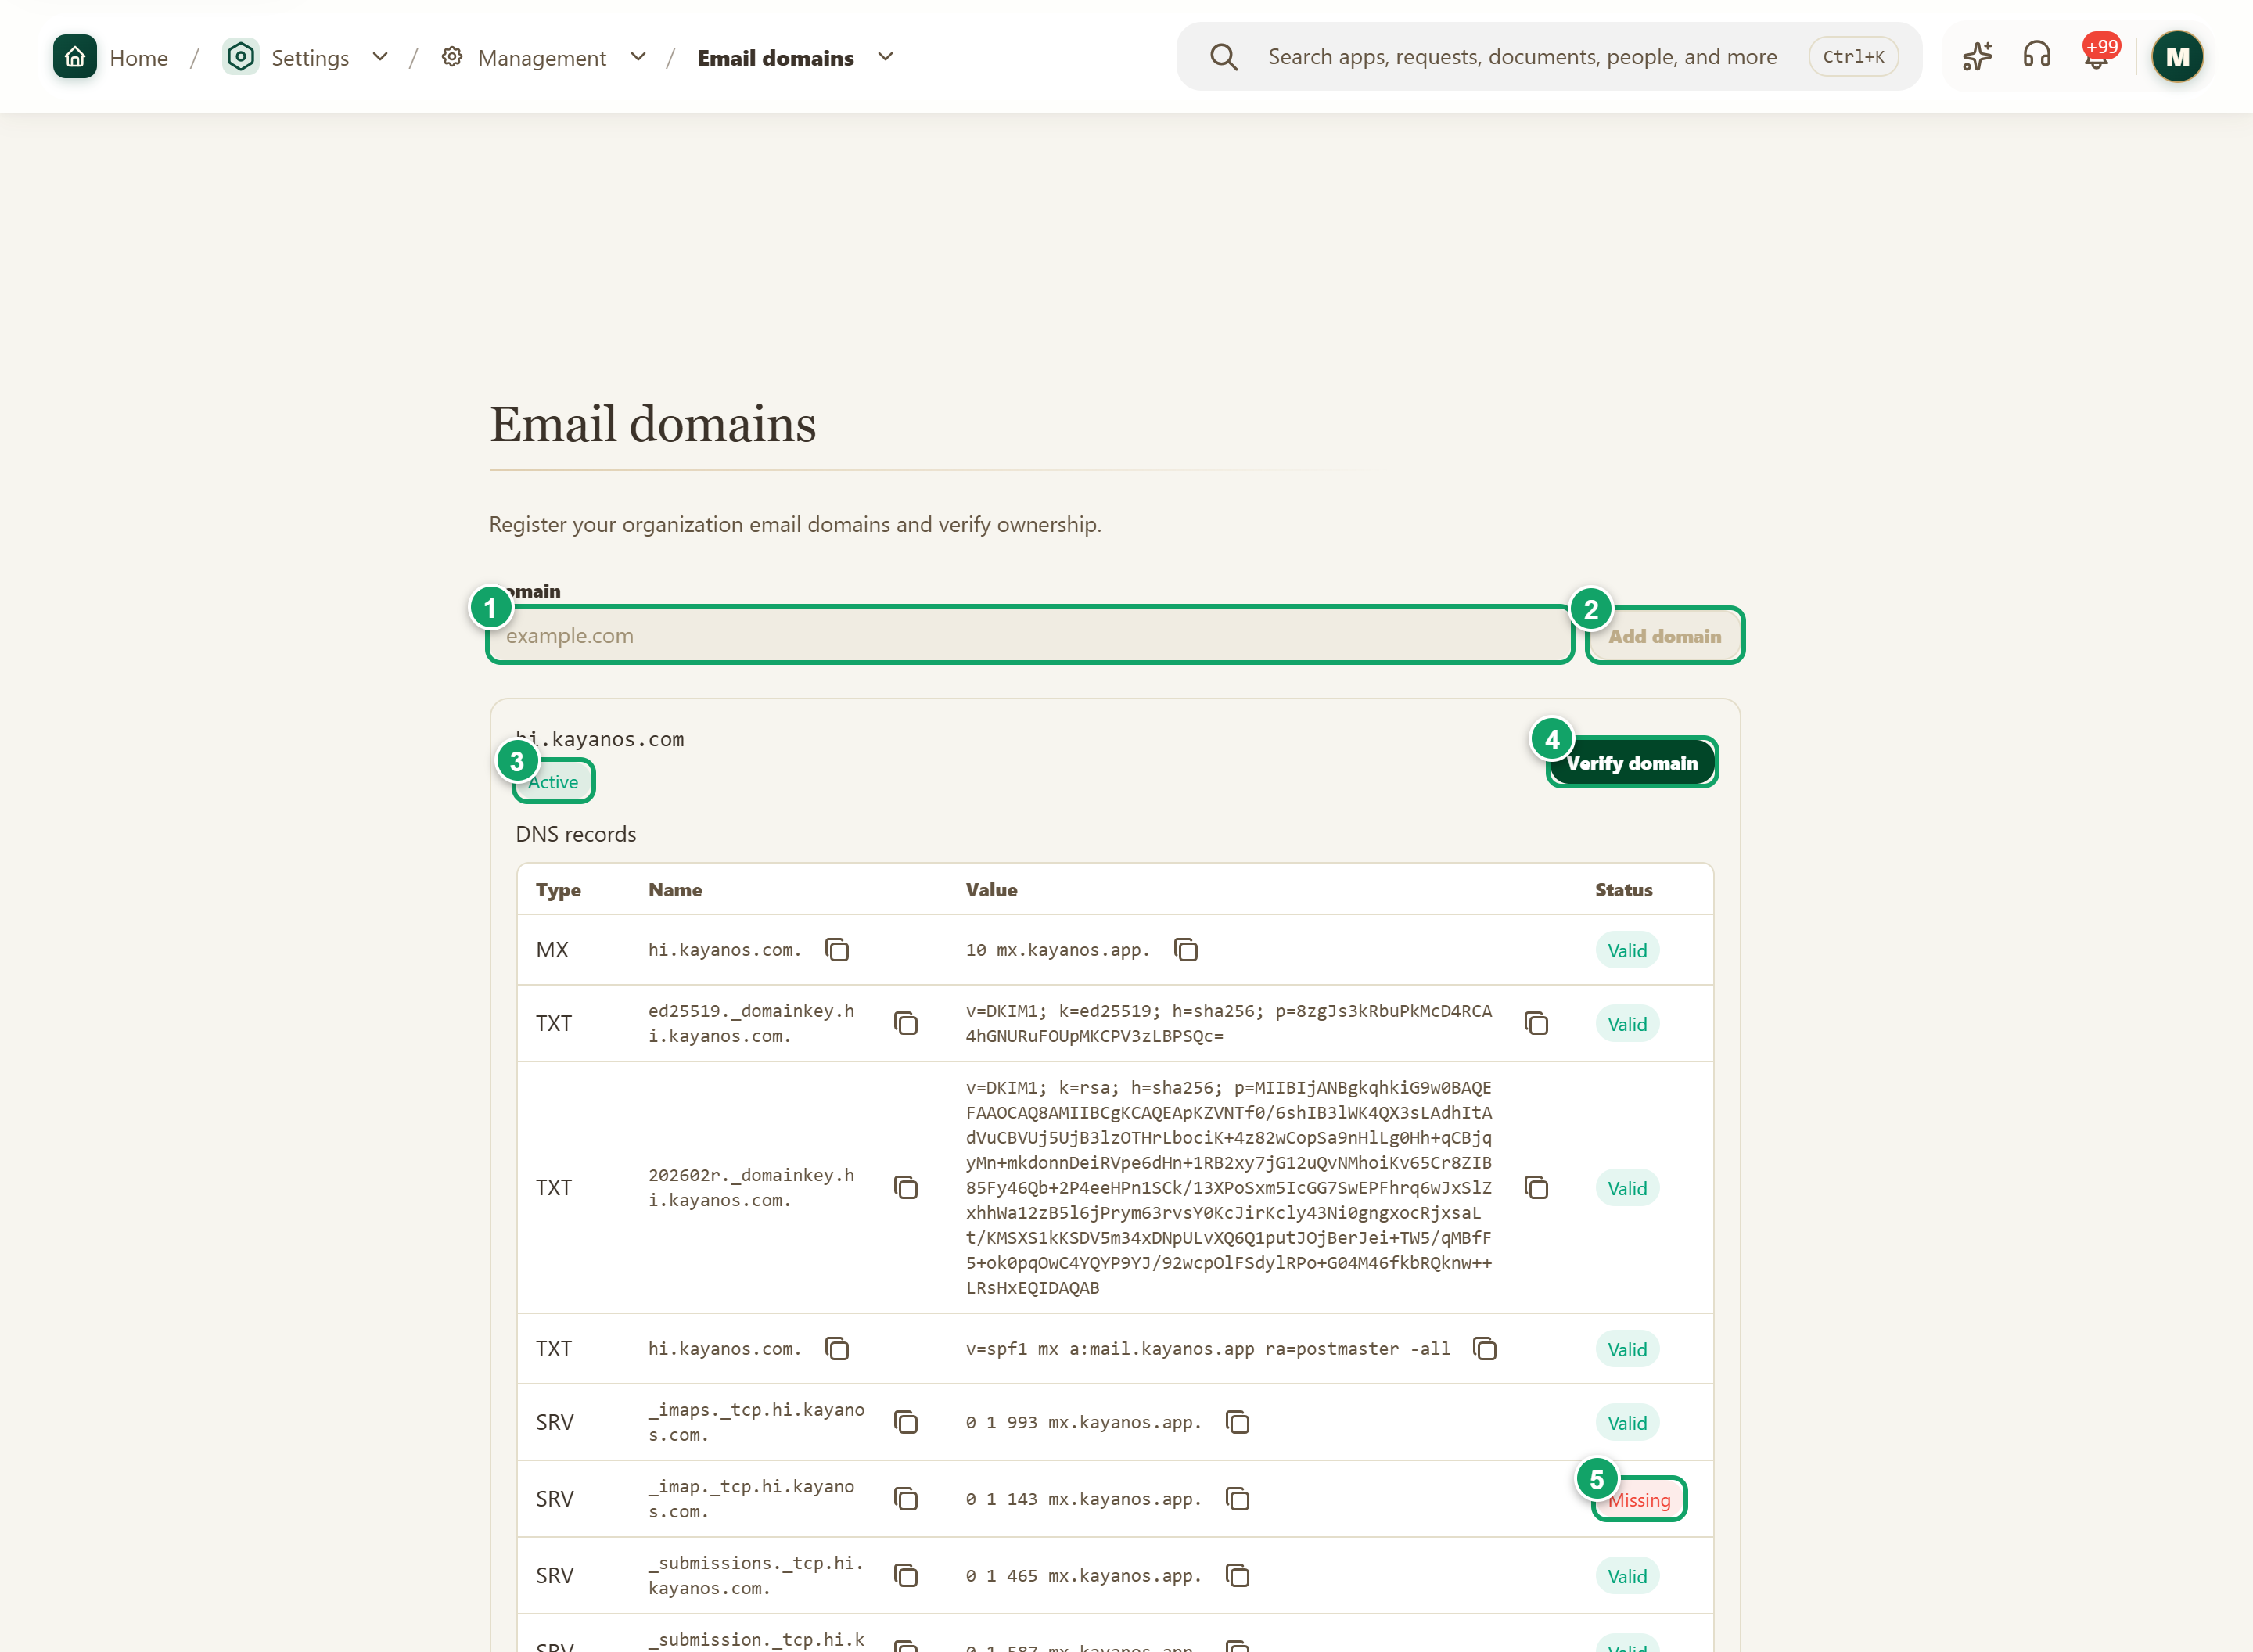
\includegraphics[width=0.95\linewidth,height=0.72\textheight,keepaspectratio]{figures/screens/ch08-email-domains-en.png}
\caption{An active domain and its DNS records}
\label{fig:settings-email-domains}
\shotnote{The image shows an active test domain and the start of its records table, including a missing record even though the domain is active; the two statuses are different. The image stops before the end of the table because the last row holds a private verification value that should not be published. ① The “Domain” field. ② “Add domain”: stays disabled until you type a domain. ③ The domain’s status. ④ “Verify domain”. ⑤ The record’s status: “Missing” means the record was not found.}
\end{figure}

\begin{figure}[H]
\centering
\begin{tikzpicture}[node distance=0.5cm]
\node[stepBox] (a) {Add the domain on this page};
\node[stepBox,below=of a] (b) {Copy the DNS records to the domain provider};
\node[stepBox,below=of b] (c) {Press Verify domain};
\node[stepBox,below=of c] (d) {The domain's status becomes Active};
\node[stepBox,below=of d] (e) {Create mailboxes on the domain};
\draw[flowsTo] (a) -- (b);
\draw[flowsTo] (b) -- (c);
\draw[flowsTo] (c) -- (d);
\draw[flowsTo] (d) -- (e);
\end{tikzpicture}
\rclegend
\caption{The stages of activating an email domain}
\label{fig:settings-email-domains-flow}
\shotnote{These stages do not advance on their own: each is an action you take, and verification cannot finish before the records are visible on the internet. So if you press the button too early and the status becomes “Error”, wait a while and try again.}
\end{figure}

\begin{table}[H]
\centering
\caption{What do you read in email domains?}
\label{tab:settings-email-domains-fields}
\begin{tabularx}{\linewidth}{R{4.2cm} Y}
\rcHeaderRow
\thh{Item} & \thh{What does it mean?}\\
“Domain” & The root domain you want to use for email. It cannot be registered if another organization already holds it.\\
Domain status & “Pending” before verification succeeds, “Active” once complete and “Error” if it fails. “Verified” appears for a moment on the way to active.\\
“DNS records” & Each record has a “Type”, “Name”, “Value” and “Status”, with a copy button beside the name and value.\\
Record status & “Valid”, “Incorrect” if the value differs, “Missing” or “Unknown”.\\
“Delete domain” & Appears only when the status is “Pending” or “Error”.\\
\end{tabularx}
\end{table}

\begin{enumerate}
\item Open “Settings”, then “Email domains”.
\item Type the domain in the “Domain” field, then press “Add domain”.
\item Copy each record’s value with the copy button and add it at the domain provider.
\item Press “Verify domain” after adding the records.
\item Check the domain’s status, then each record’s status in the table.
\end{enumerate}

\textbf{Check:} The “Active” status and a success message appear. The button checks the ownership record only, so review the other records yourself and correct any marked “Missing” or “Incorrect” if sending or receiving fails. Note that verifying again after removing the ownership record turns the status to “Error”.

\clearpage
\section{Email signatures}
\label{sec:settings-feature-email-signatures}

A signature is the part at the end of a message that carries the sender’s name, position and contact details. Here you design one template that each member’s details fill automatically, so your messages look consistent without members writing their own. A disclaimer is a shared legal text added to outgoing messages.

Use this page when adopting an organization signature or changing your identity. Only the organization owner manages it, and others see a message saying so. Each member manages their personal signatures from “Manage signatures…” when writing a message, unless the organization signature is enforced for them.

\begin{rcnote}[Example: Horizon]
The system administrator creates a Horizon template at ② and publishes it, then adds a rule making it enforced for everyone. When Omar Haddad sends a new email, his name and position appear automatically, while the card at ④ shows members with missing details.
\end{rcnote}
\begin{figure}[H]
\centering
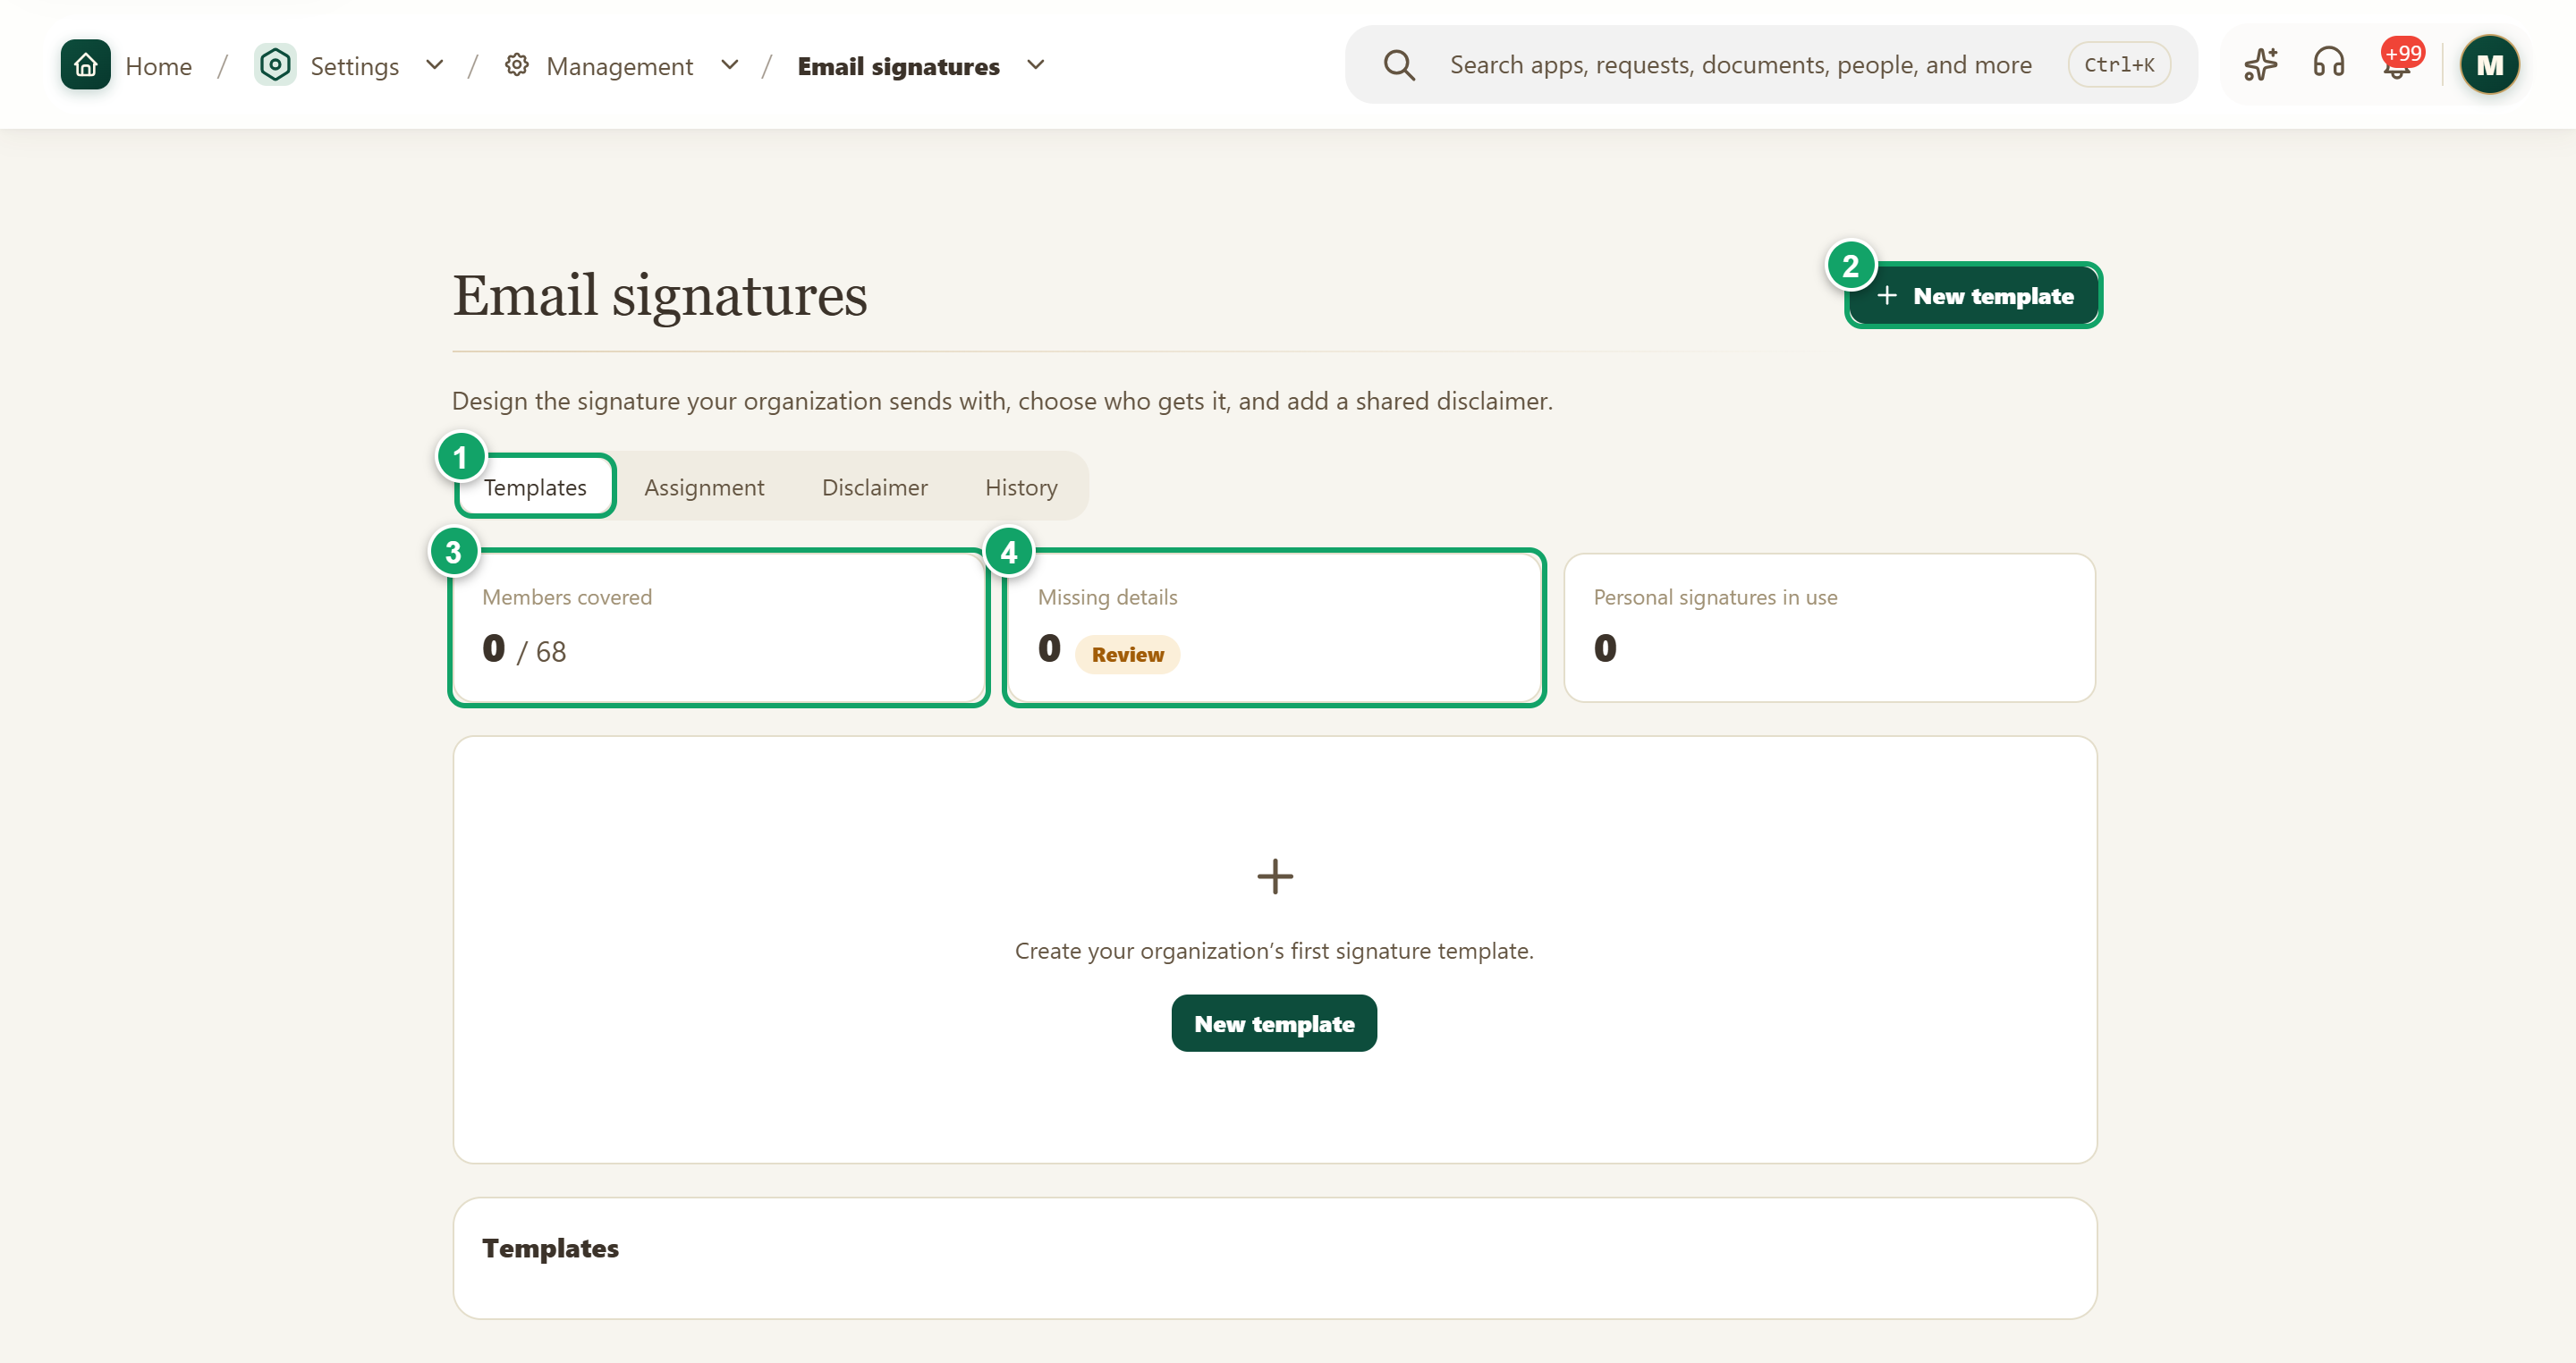
\includegraphics[width=0.95\linewidth,height=0.72\textheight,keepaspectratio]{figures/screens/ch08-email-signatures-en.png}
\caption{The Templates tab}
\label{fig:settings-email-signatures}
\shotnote{The image shows the starting point in the test organization, with no template yet, so no member is covered. The cards help you follow coverage after publishing. ① “Templates”. ② “New template”. ③ “Members covered”: how many members a signature applies to, out of all members. ④ “Missing details”: opens a review of members lacking a field.}
\end{figure}

\begin{figure}[H]
\centering
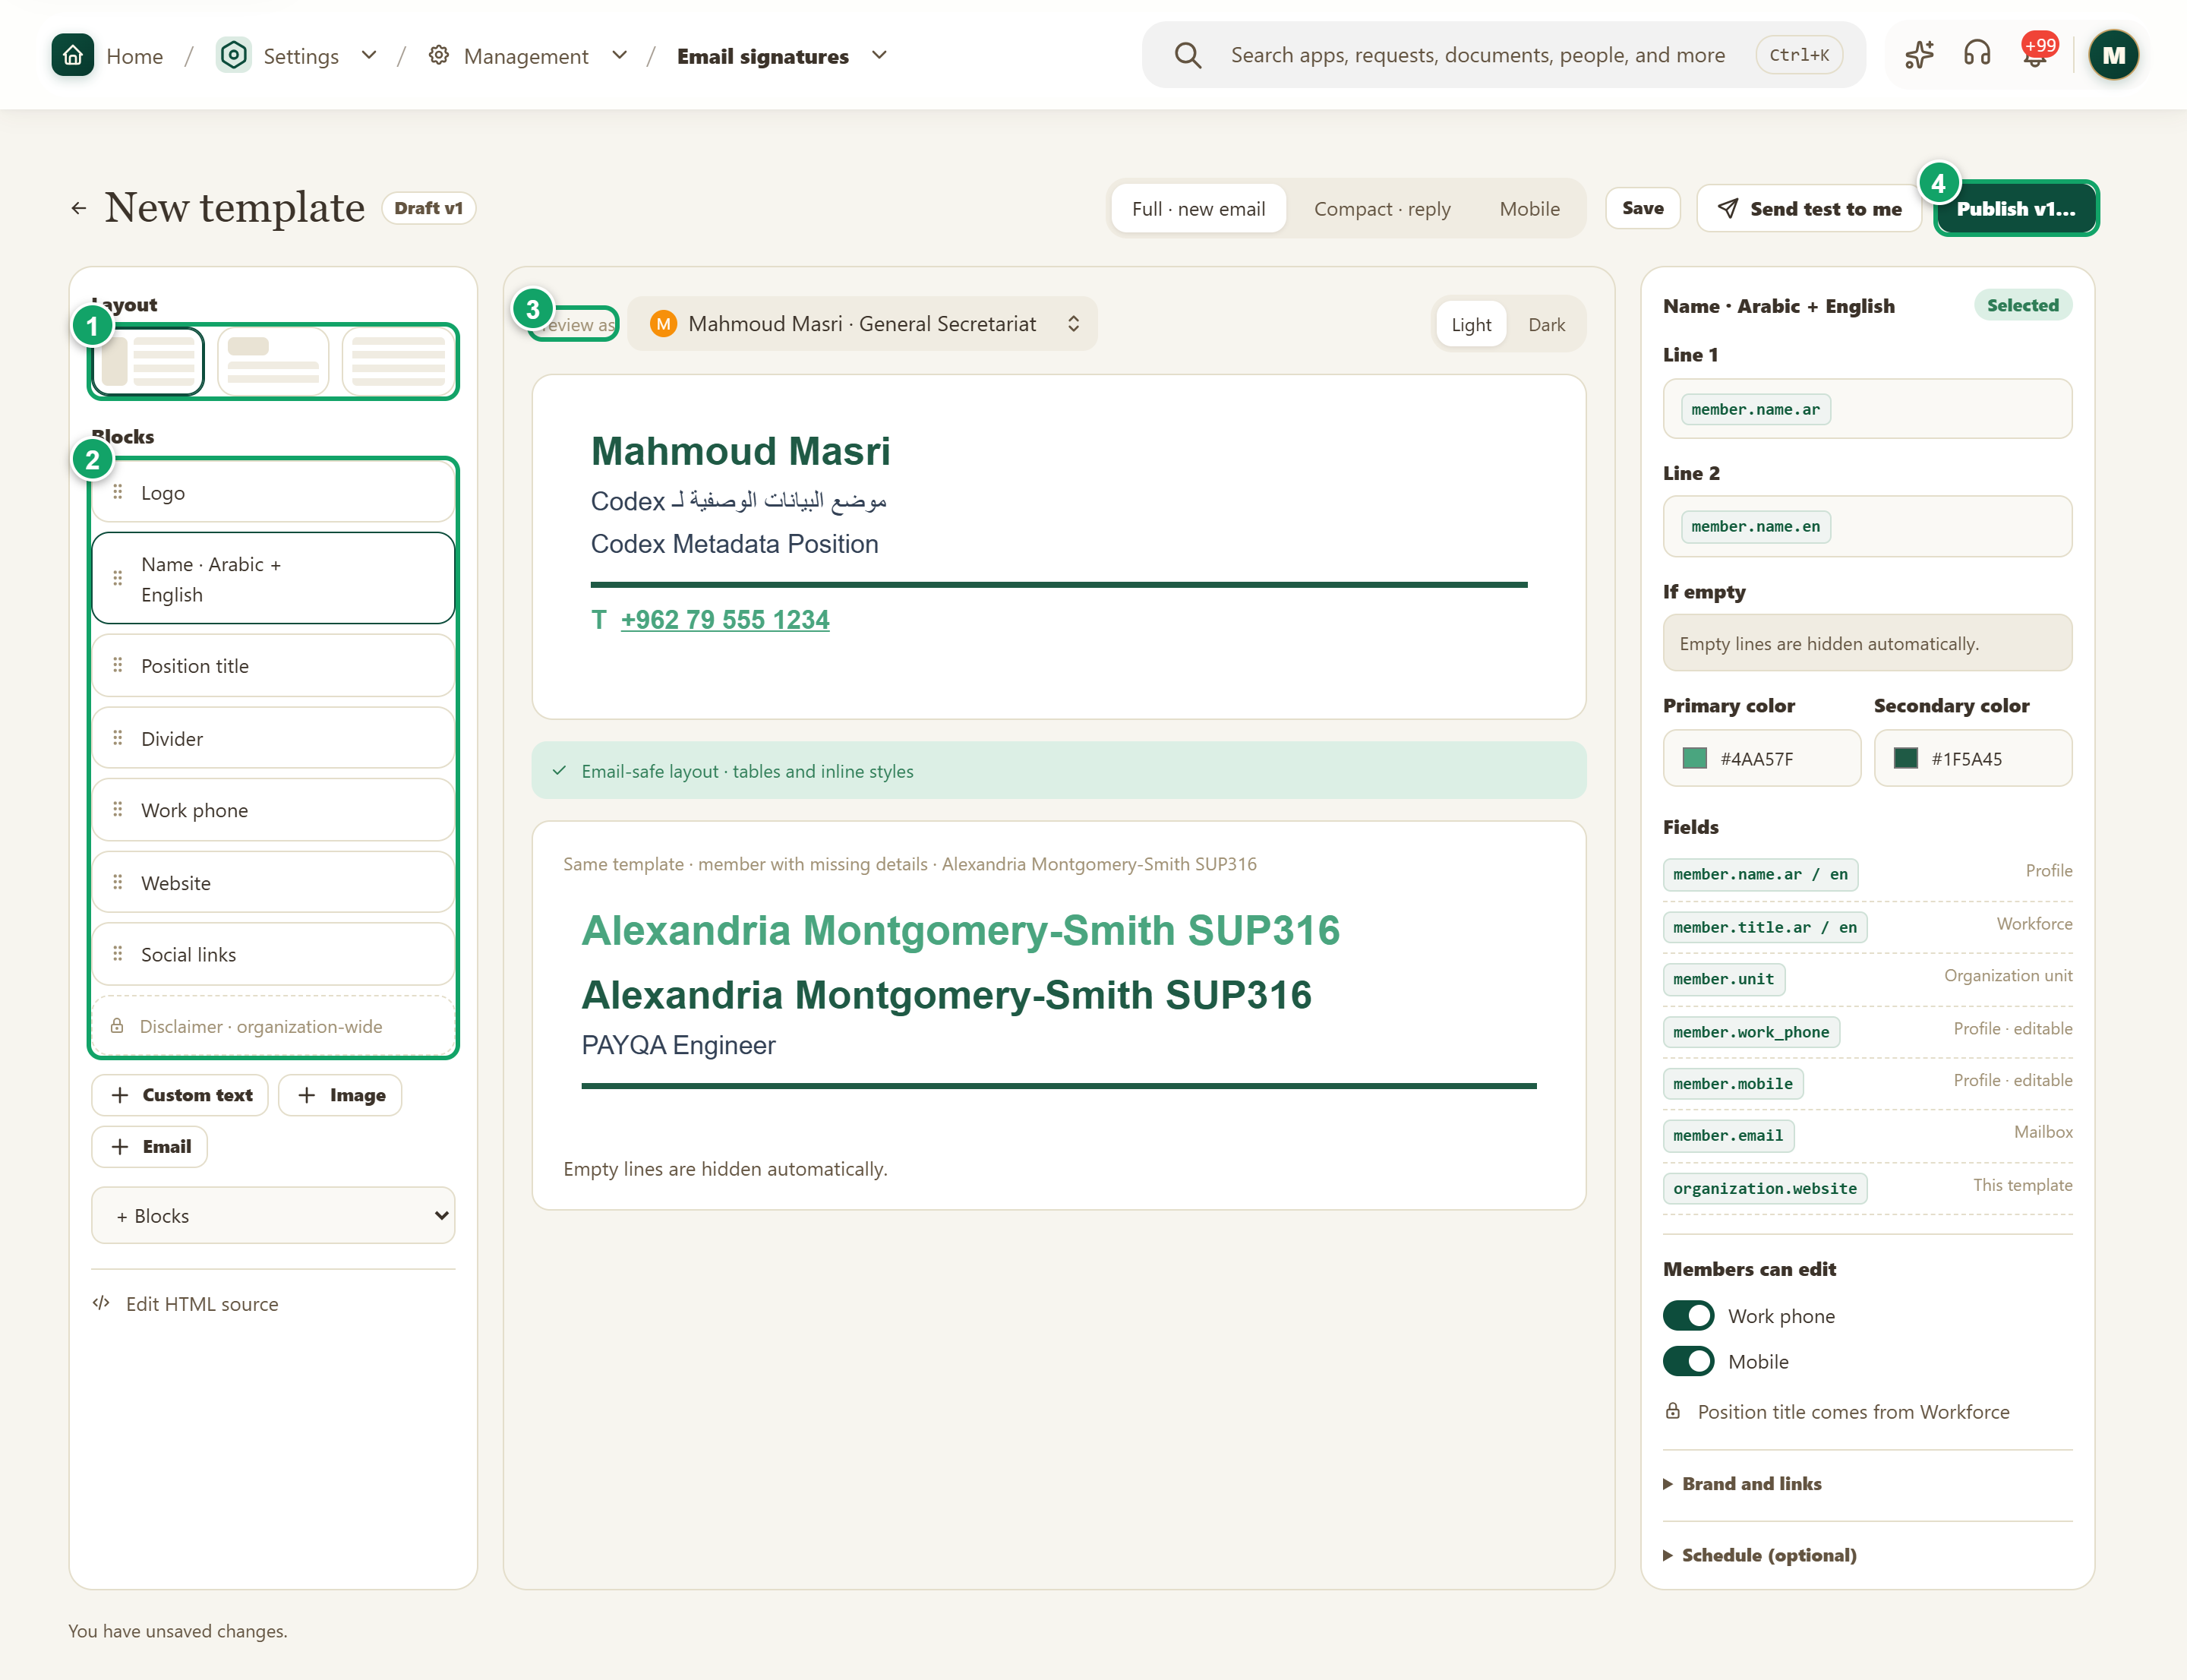
\includegraphics[width=0.95\linewidth,height=0.72\textheight,keepaspectratio]{figures/screens/ch08-email-signatures-designer-en.png}
\caption{The signature designer}
\label{fig:settings-email-signatures-designer}
\shotnote{“New template” opens this designer; the template shown is a trial that was not saved. The preview shows the signature with the details of a member of the test organization, then with a member whose details are incomplete, so you see empty lines disappear automatically. ① “Layout”. ② “Blocks”: what the signature shows and in what order. ③ “Preview as”: chooses whose details you preview. ④ “Publish v1…”: starts the details review before publishing the version.}
\end{figure}

\begin{figure}[H]
\centering
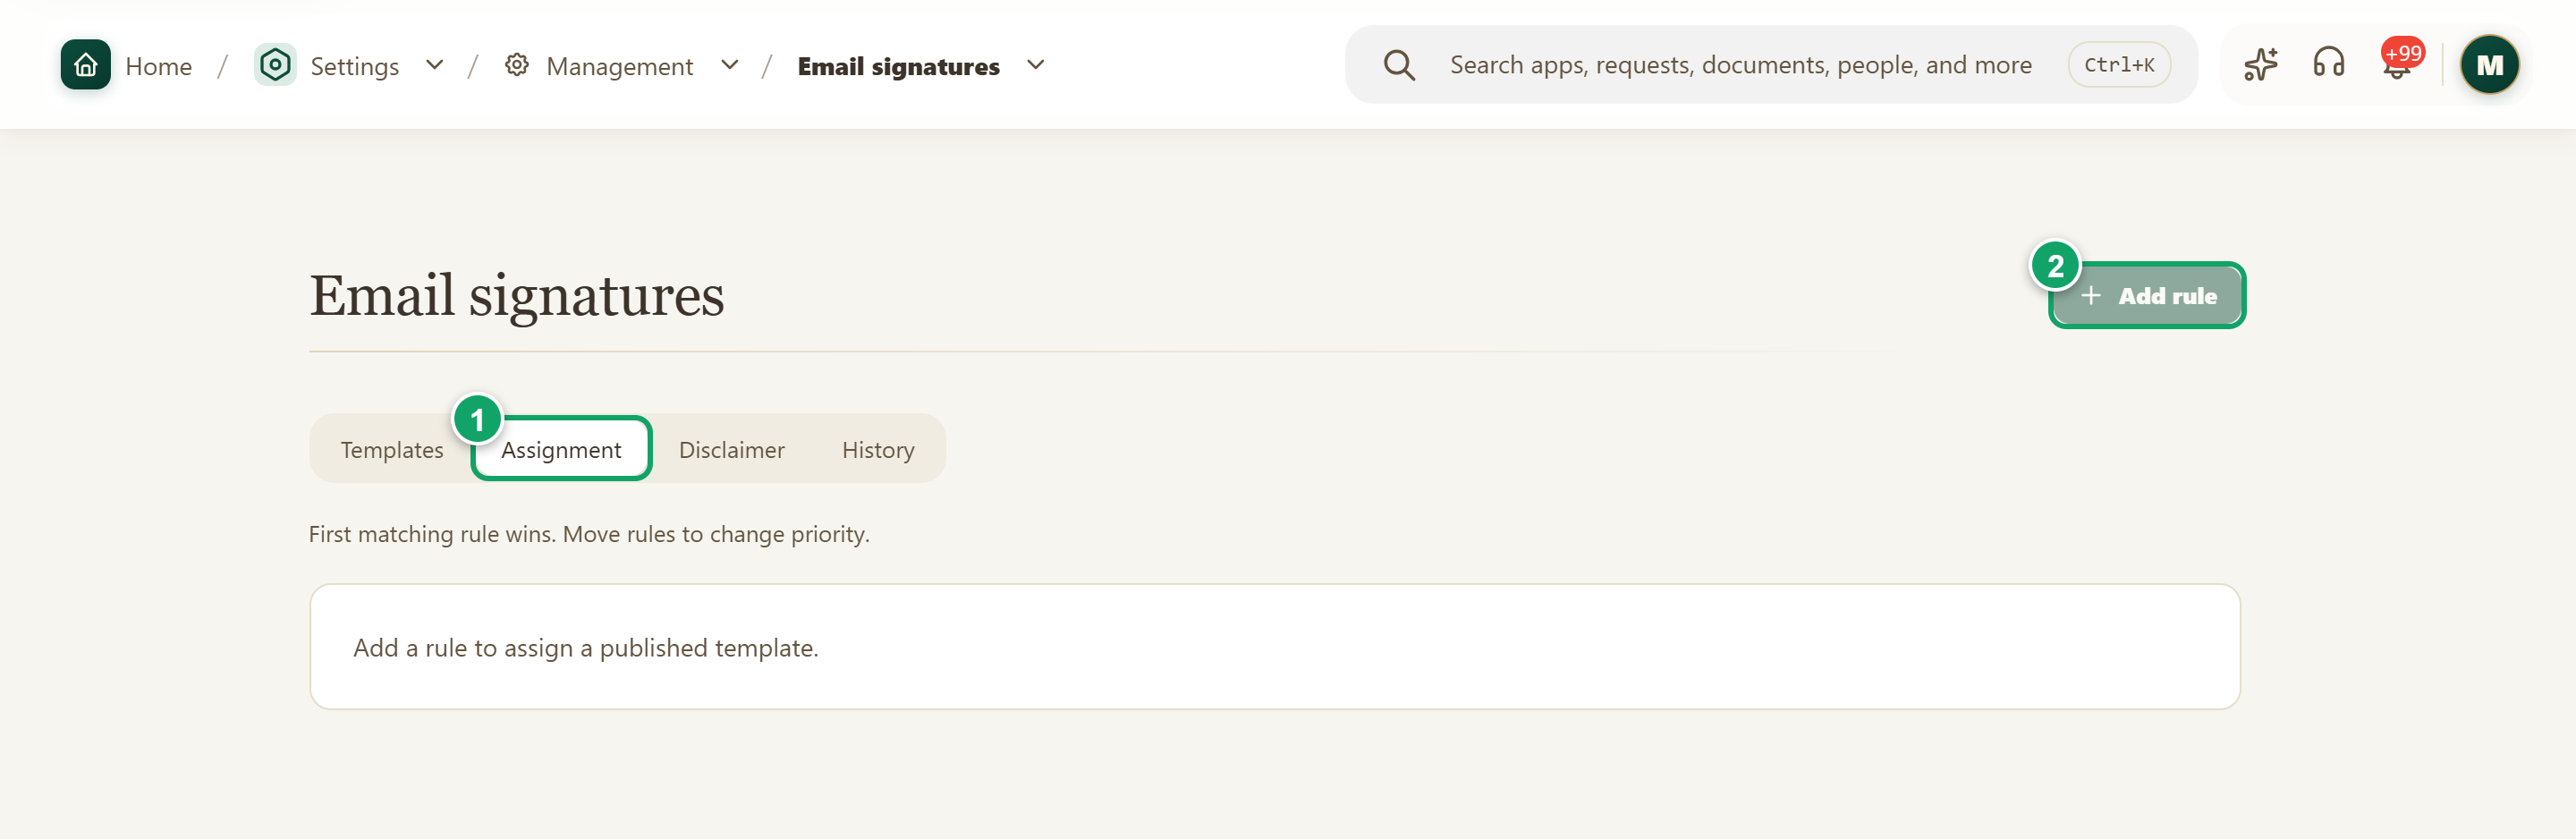
\includegraphics[width=0.95\linewidth,height=0.72\textheight,keepaspectratio]{figures/screens/ch08-email-signatures-assignment-en.png}
\caption{The Assignment tab}
\label{fig:settings-email-signatures-assignment}
\shotnote{Assignment decides who uses each template, and a template does not reach members without a rule. The button is disabled in this image because the test organization has no template yet. ① “Assignment”. ② “Add rule”.}
\end{figure}

\begin{figure}[H]
\centering
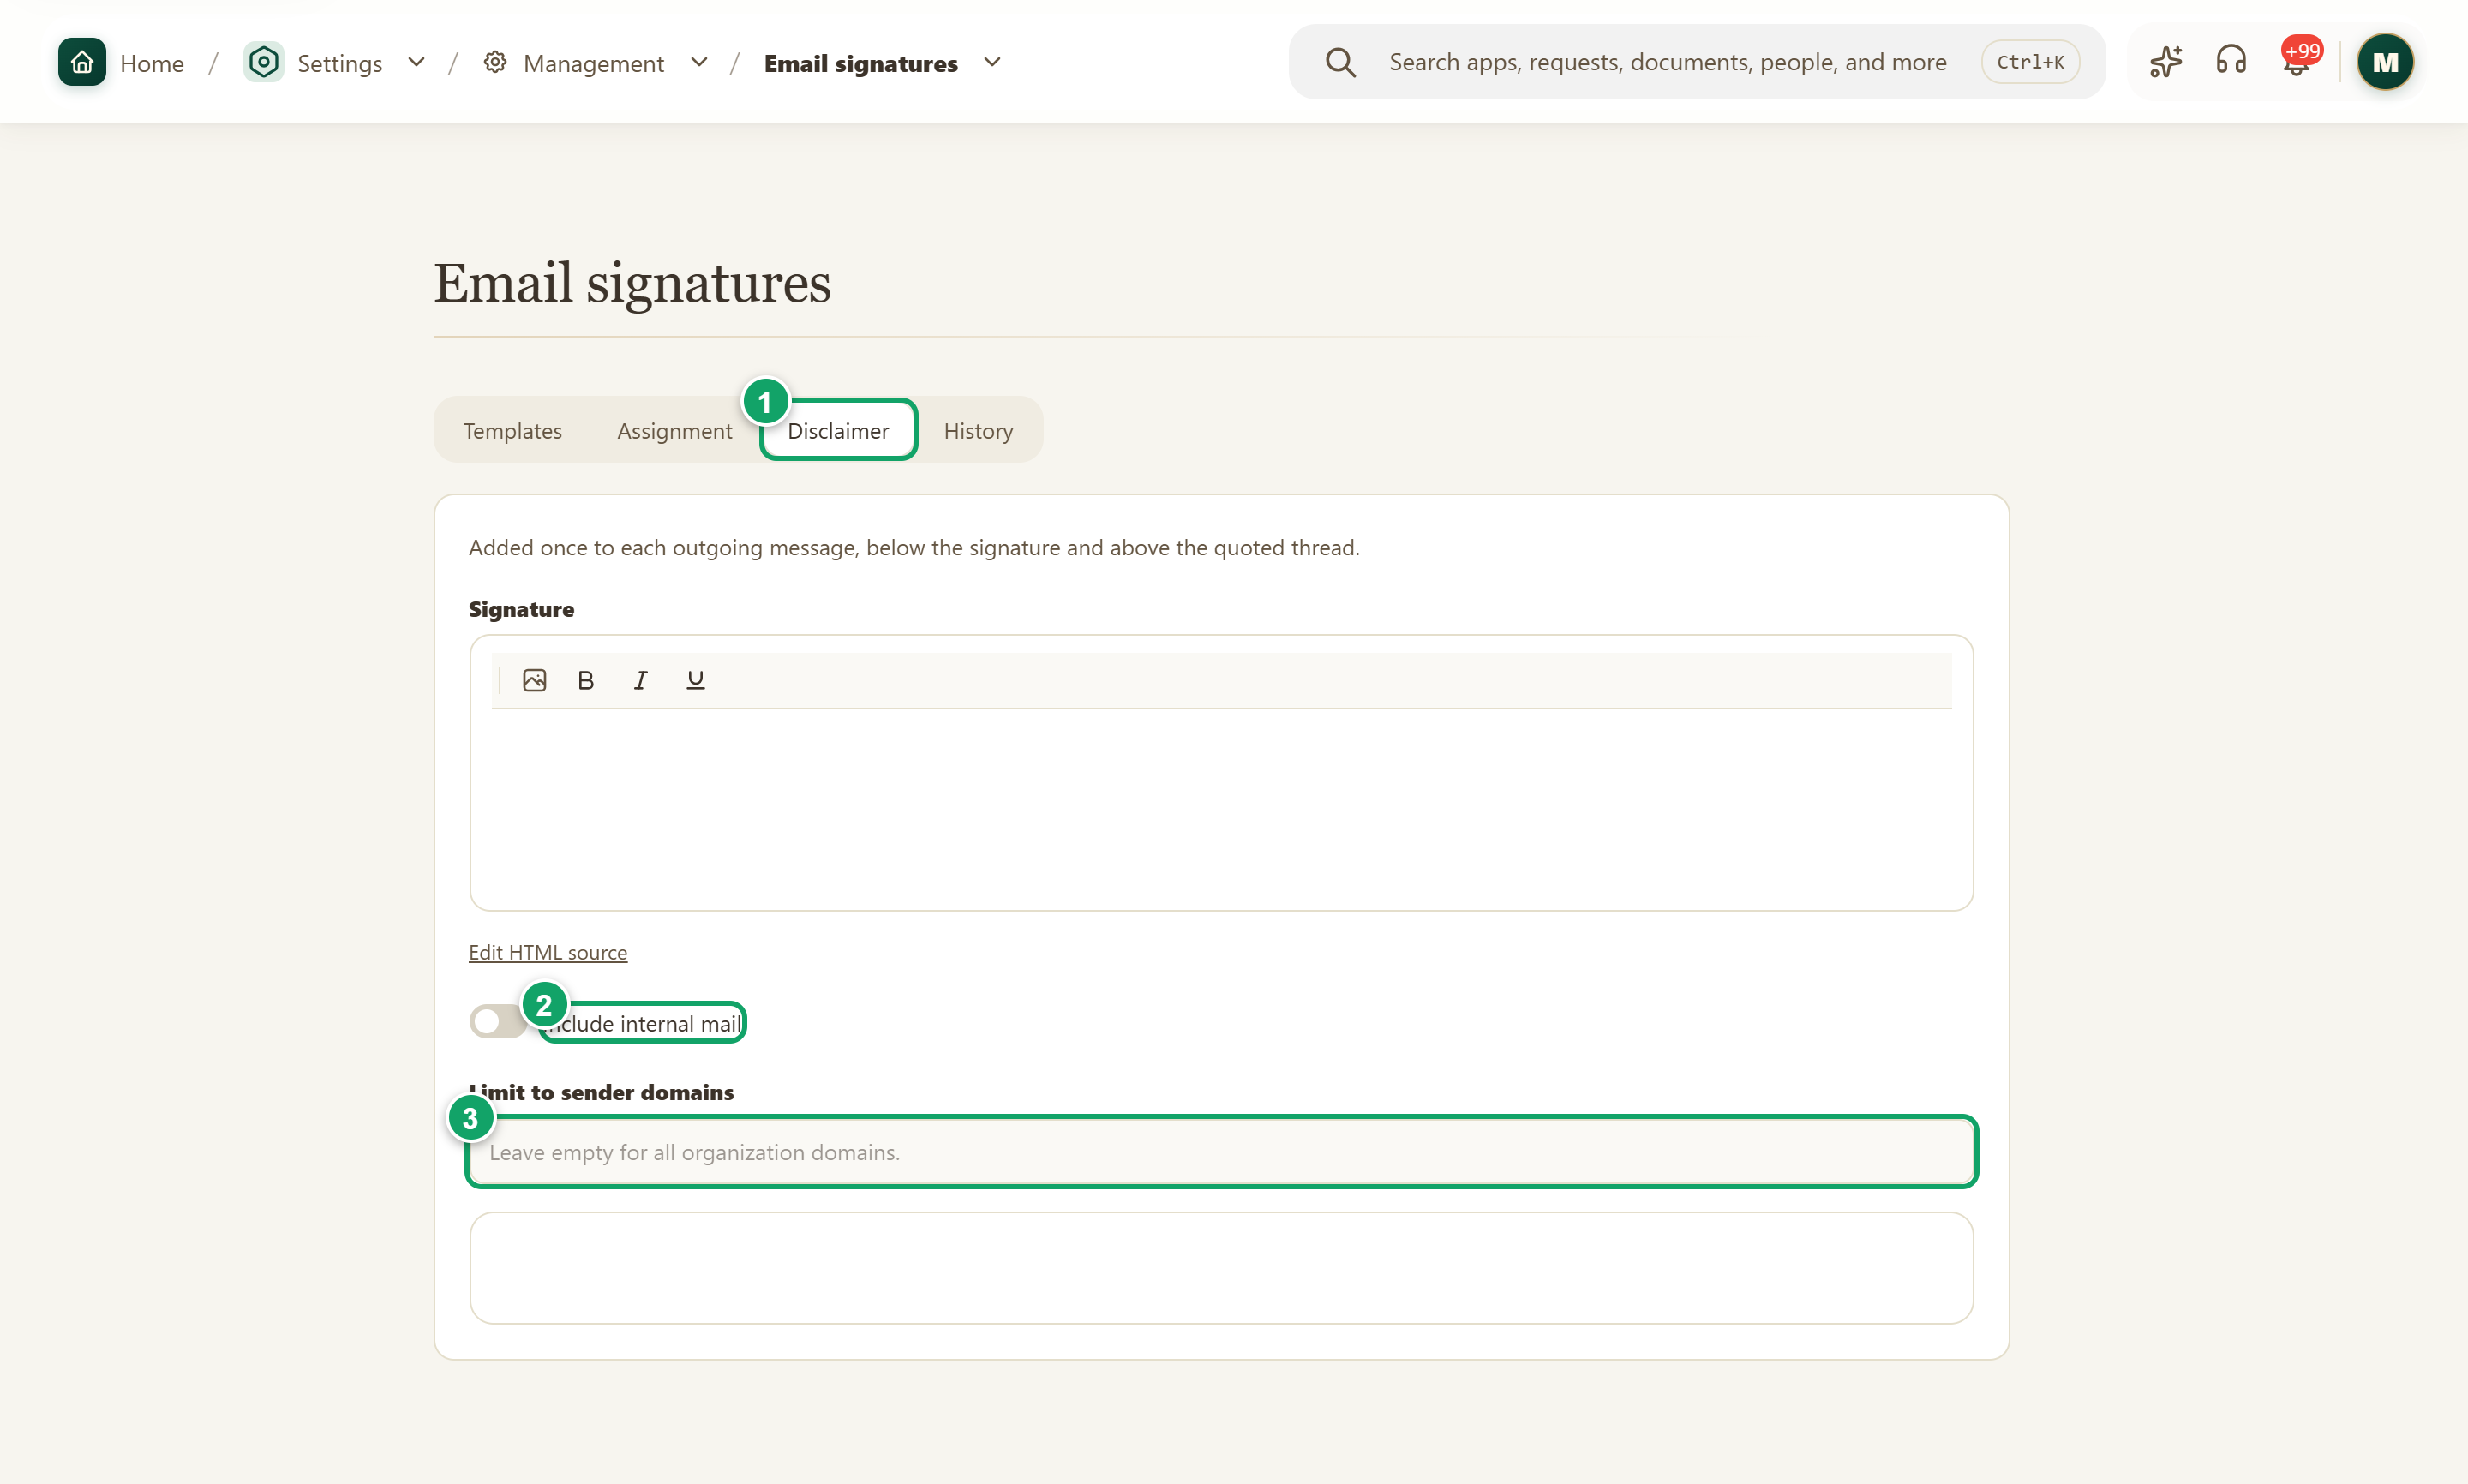
\includegraphics[width=0.95\linewidth,height=0.72\textheight,keepaspectratio]{figures/screens/ch08-email-signatures-disclaimer-en.png}
\caption{The Disclaimer tab}
\label{fig:settings-email-signatures-disclaimer}
\shotnote{This text is added once to each outgoing message, below the signature and above the quoted thread, so it does not repeat in replies. The text is empty in the test organization. ① “Disclaimer”. ② “Include internal mail”: also adds the text to messages between members. ③ The “Limit to sender domains” field: leave it empty to cover all your organization’s domains.}
\end{figure}

\begin{figure}[H]
\centering
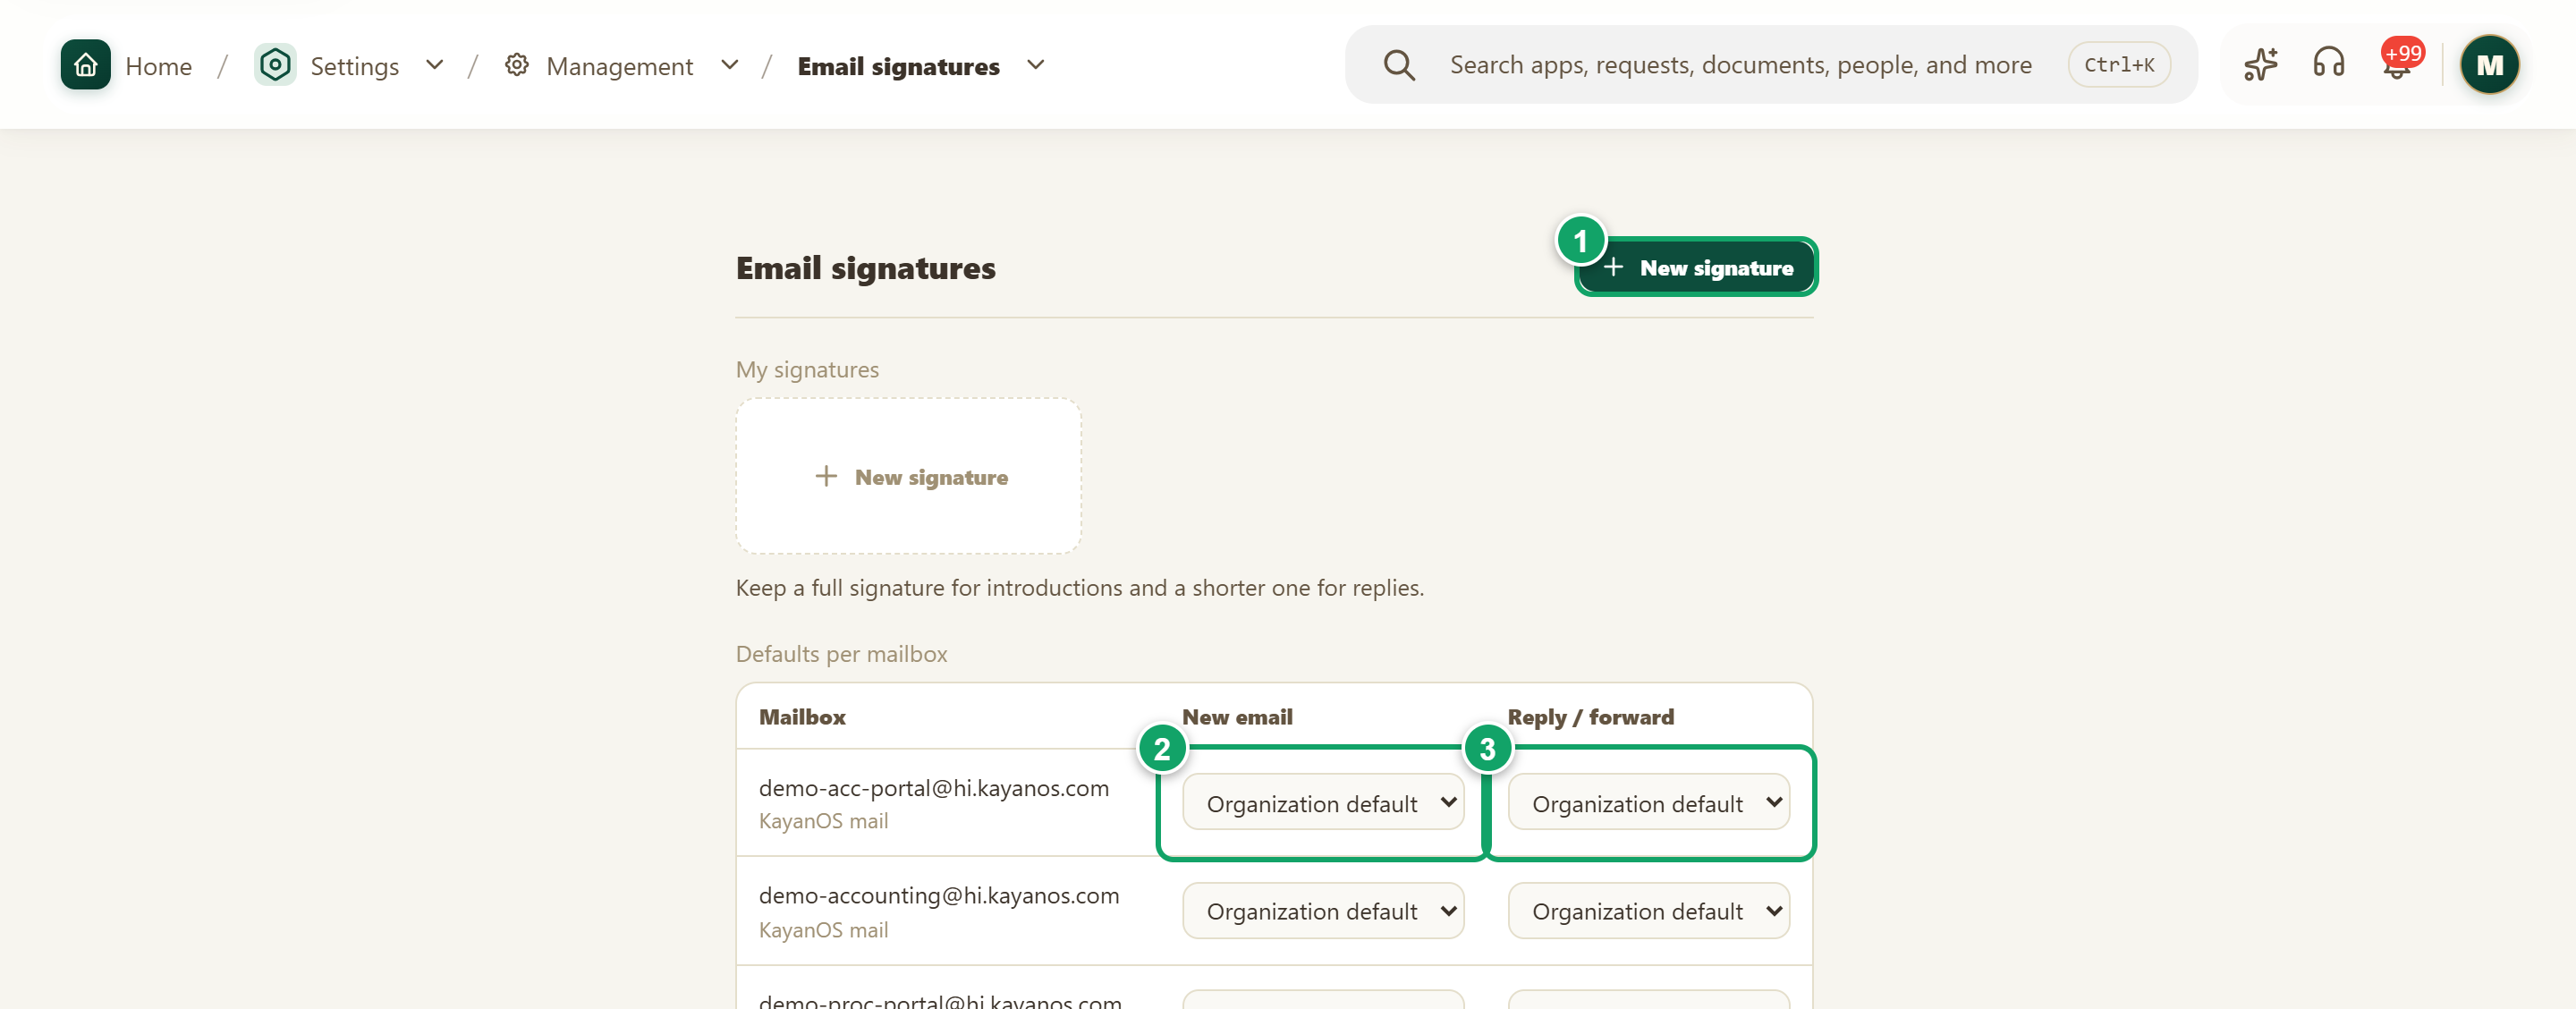
\includegraphics[width=0.95\linewidth,height=0.72\textheight,keepaspectratio]{figures/screens/ch08-email-signatures-personal-en.png}
\caption{My signatures}
\label{fig:settings-email-signatures-personal}
\shotnote{This is the page a member sees for themselves, where they can keep a full signature and a shorter one for replies. Each row belongs to a mailbox, so settings can differ from one mailbox to another. ① “New signature”. ② The default signature for new emails from this mailbox. ③ The default signature for replies and forwards.}
\end{figure}

\begin{table}[H]
\centering
\caption{What do you record in email signatures?}
\label{tab:settings-email-signatures-fields}
\begin{tabularx}{\linewidth}{R{4.2cm} Y}
\rcHeaderRow
\thh{Section} & \thh{What do you record?}\\
“Templates” & The name, “Layout”, “Blocks”, colors, “Brand and links”, “Schedule (optional)”, and the fields allowed under “Members can edit”. Each template has three versions: “Full · new email”, “Compact · reply” and “Mobile”.\\
“Assignment” & Rules with “Applies to”, “Template” and “Mode”, and the version used for new emails and replies. The first matching rule wins, so order them by priority.\\
“Mode” & “Enforced”: always added and members cannot change it. “Default”: preselected and members can switch. “Optional”: available in the signature menu.\\
“Disclaimer” & The disclaimer text, “Include internal mail” and “Limit to sender domains”.\\
“History” & Published versions, with “Restore as a new version”.\\
\end{tabularx}
\end{table}

\begin{enumerate}
\item Open “Settings”, then “Email signatures”, and press “New template”.
\item Choose the layout and blocks, then check the preview with more than one member.
\item Press “Send test to me” if you want to see the signature in your mailbox.
\item Press the “Publish” button, review the members with missing details, then finish publishing.
\item Open “Assignment”, press “Add rule”, set who it applies to, the template and the mode, then save.
\end{enumerate}

\textbf{Check:} The “Members covered” count changes on the “Templates” tab and the version appears in “History”. The published version applies at the next send, including unsent drafts, so confirm it on the next message a member sends.

\clearpage
\section{Short link domains}
\label{sec:settings-feature-short-links}

A short link is a brief address that leads to a long page and fits easily inside a message. This page lets those links carry your organization’s name instead of the platform’s general address, which reassures whoever receives them. A custom domain here is a sub-address you dedicate to these links, such as one starting with the word links.

This page is optional: when no domain is active, links are created on your organization’s platform address. Only the organization owner manages it, and others see a message asking them to contact the owner. Adding a domain follows the same stages explained on the email domains page (\ref{sec:settings-feature-email-domains}).

\begin{rcnote}[Example: Horizon]
The system administrator wants links in Horizon’s messages to carry its name, so he types a subdomain at ① and presses ②. He then adds the two records at the domain provider and presses ④, and the status at ③ turns “Active”.
\end{rcnote}
\begin{figure}[H]
\centering
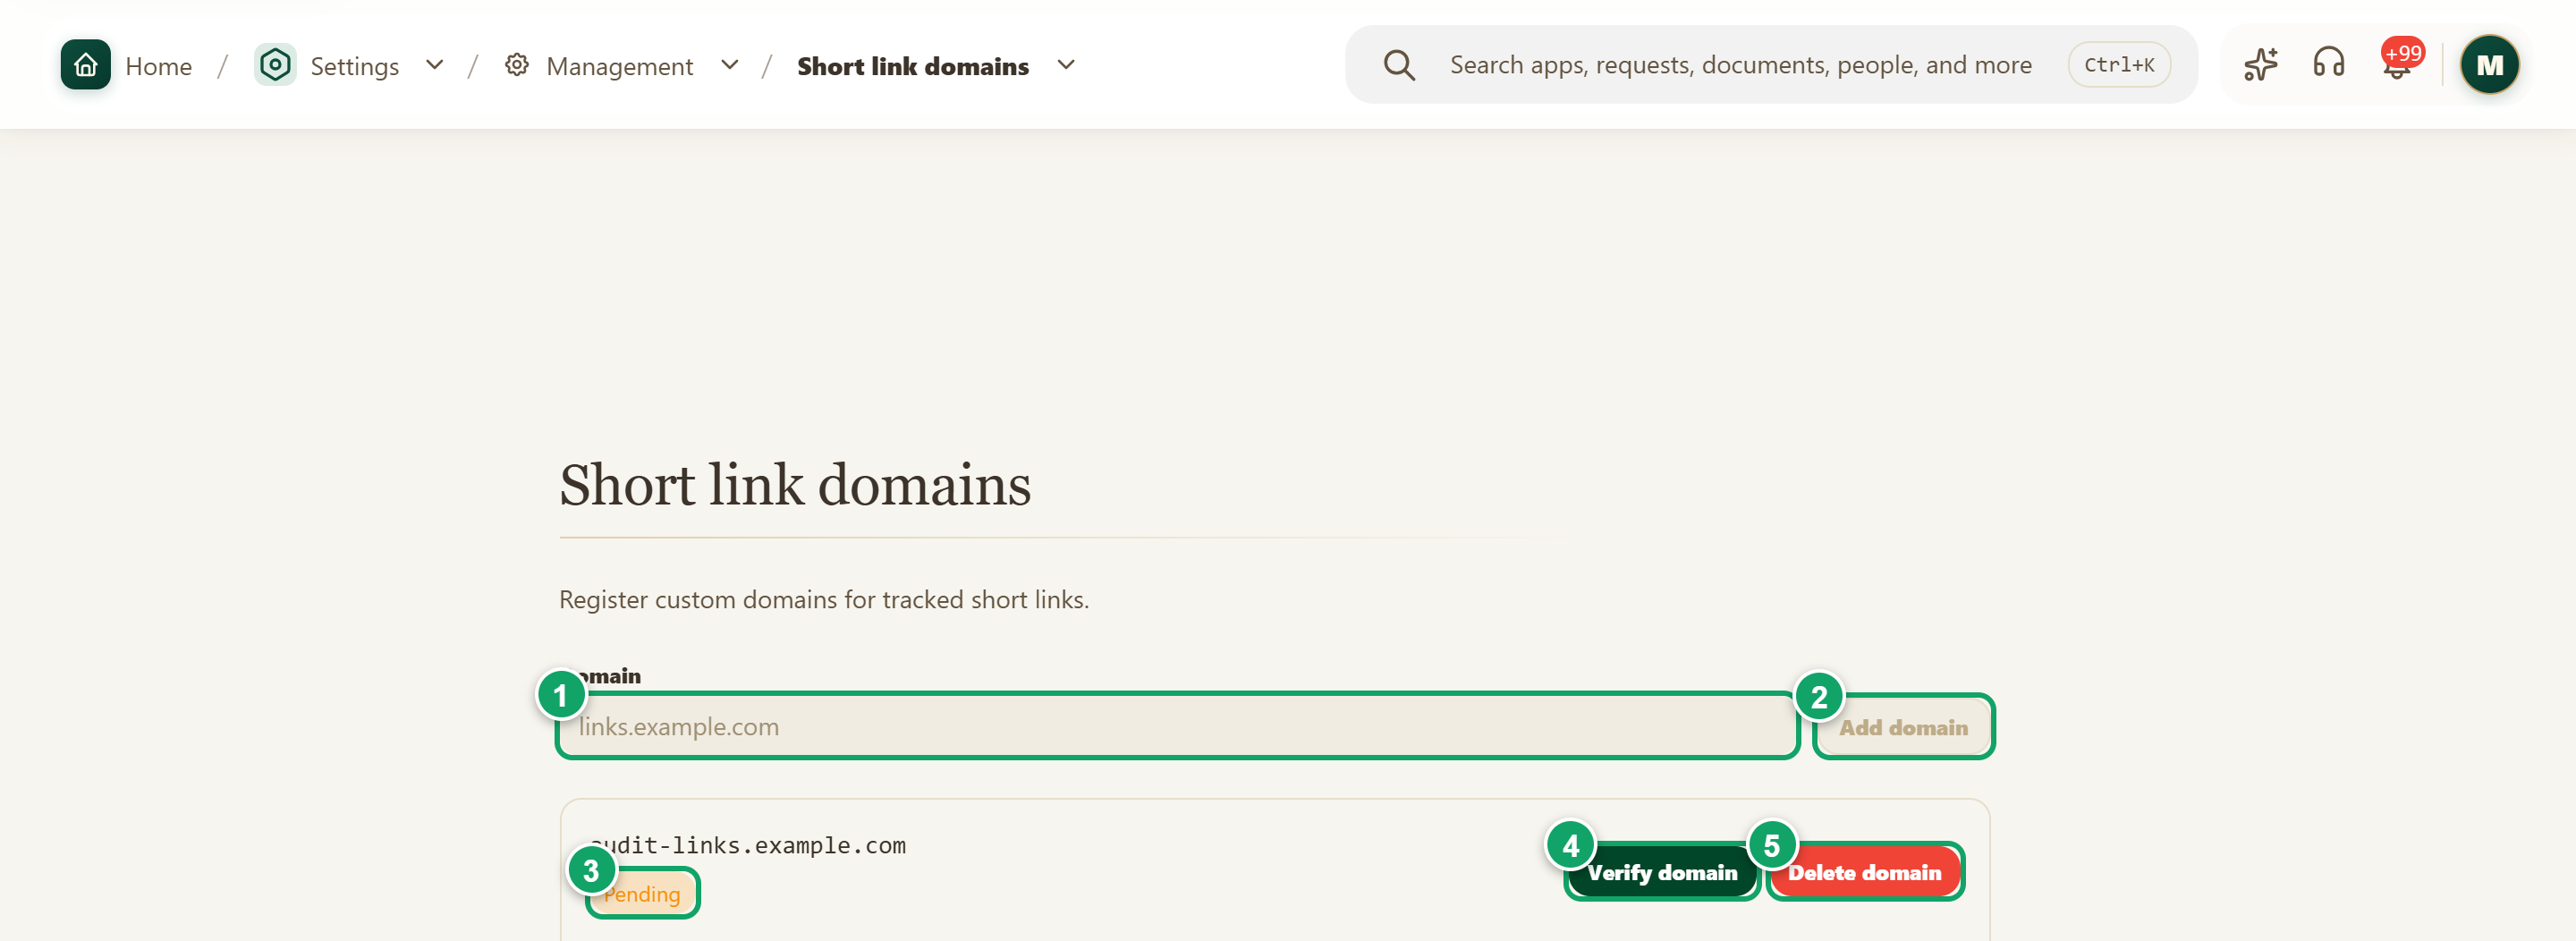
\includegraphics[width=0.95\linewidth,height=0.72\textheight,keepaspectratio]{figures/screens/ch08-short-links-en.png}
\caption{A pending short link domain}
\label{fig:settings-short-links}
\shotnote{The image shows a test domain whose verification is not complete. It stops before the records table because the first row holds a private verification value; the table’s layout is explained on the email domains page. ① The “Domain” field. ② “Add domain”. ③ The domain’s status. ④ “Verify domain”. ⑤ “Delete domain”.}
\end{figure}

\begin{table}[H]
\centering
\caption{What do you read in short link domains?}
\label{tab:settings-short-links-fields}
\begin{tabularx}{\linewidth}{R{4.2cm} Y}
\rcHeaderRow
\thh{Item} & \thh{What does it mean?}\\
“Domain” & The subdomain you dedicate to links.\\
TXT record & Proves you own the domain; this is the record the verify button checks.\\
CNAME record & Points the domain to the address the page shows, so links work when opened.\\
Domain status & “Pending”, “Active” or “Error”, and “Disabled” after a domain is deleted.\\
\end{tabularx}
\end{table}

\begin{enumerate}
\item Open “Settings”, then “Short link domains”.
\item Type the domain, then press “Add domain”.
\item Add the two records shown under “DNS records” at the domain provider.
\item Press “Verify domain”.
\end{enumerate}

\textbf{Check:} The status becomes “Active” and “Valid” appears beside both records. Then create a short link and open it: verification does not check the CNAME record, so a link may not work if that record is missing.

\clearpage
\section{WhatsApp accounts}
\label{sec:settings-feature-whatsapp}

This page links WhatsApp numbers to the organization so their conversations appear in the system’s chat. Linking is like opening WhatsApp on an extra device: the number stays on your phone, and the system connects as a linked device. A personal account belongs to one member, while a shared account belongs to a team.

These accounts differ from “WhatsApp · official number” on the messages page (\ref{sec:settings-feature-messages}): that number sends applicant messages, while the numbers here are for conversations. The page lists the accounts you may see, and the link button appears only for those allowed to create an account. Come back to this page when an account drops out of chat.

\begin{rcnote}[Example: Horizon]
Horizon’s system administrator links the Aleppo branch number as a shared account with a clear name, so Sarah Al-Khatib and Omar Haddad can follow its conversations. When messages stop arriving, he opens the page and checks the card at ④, then the account’s status in the table.
\end{rcnote}
\begin{figure}[H]
\centering
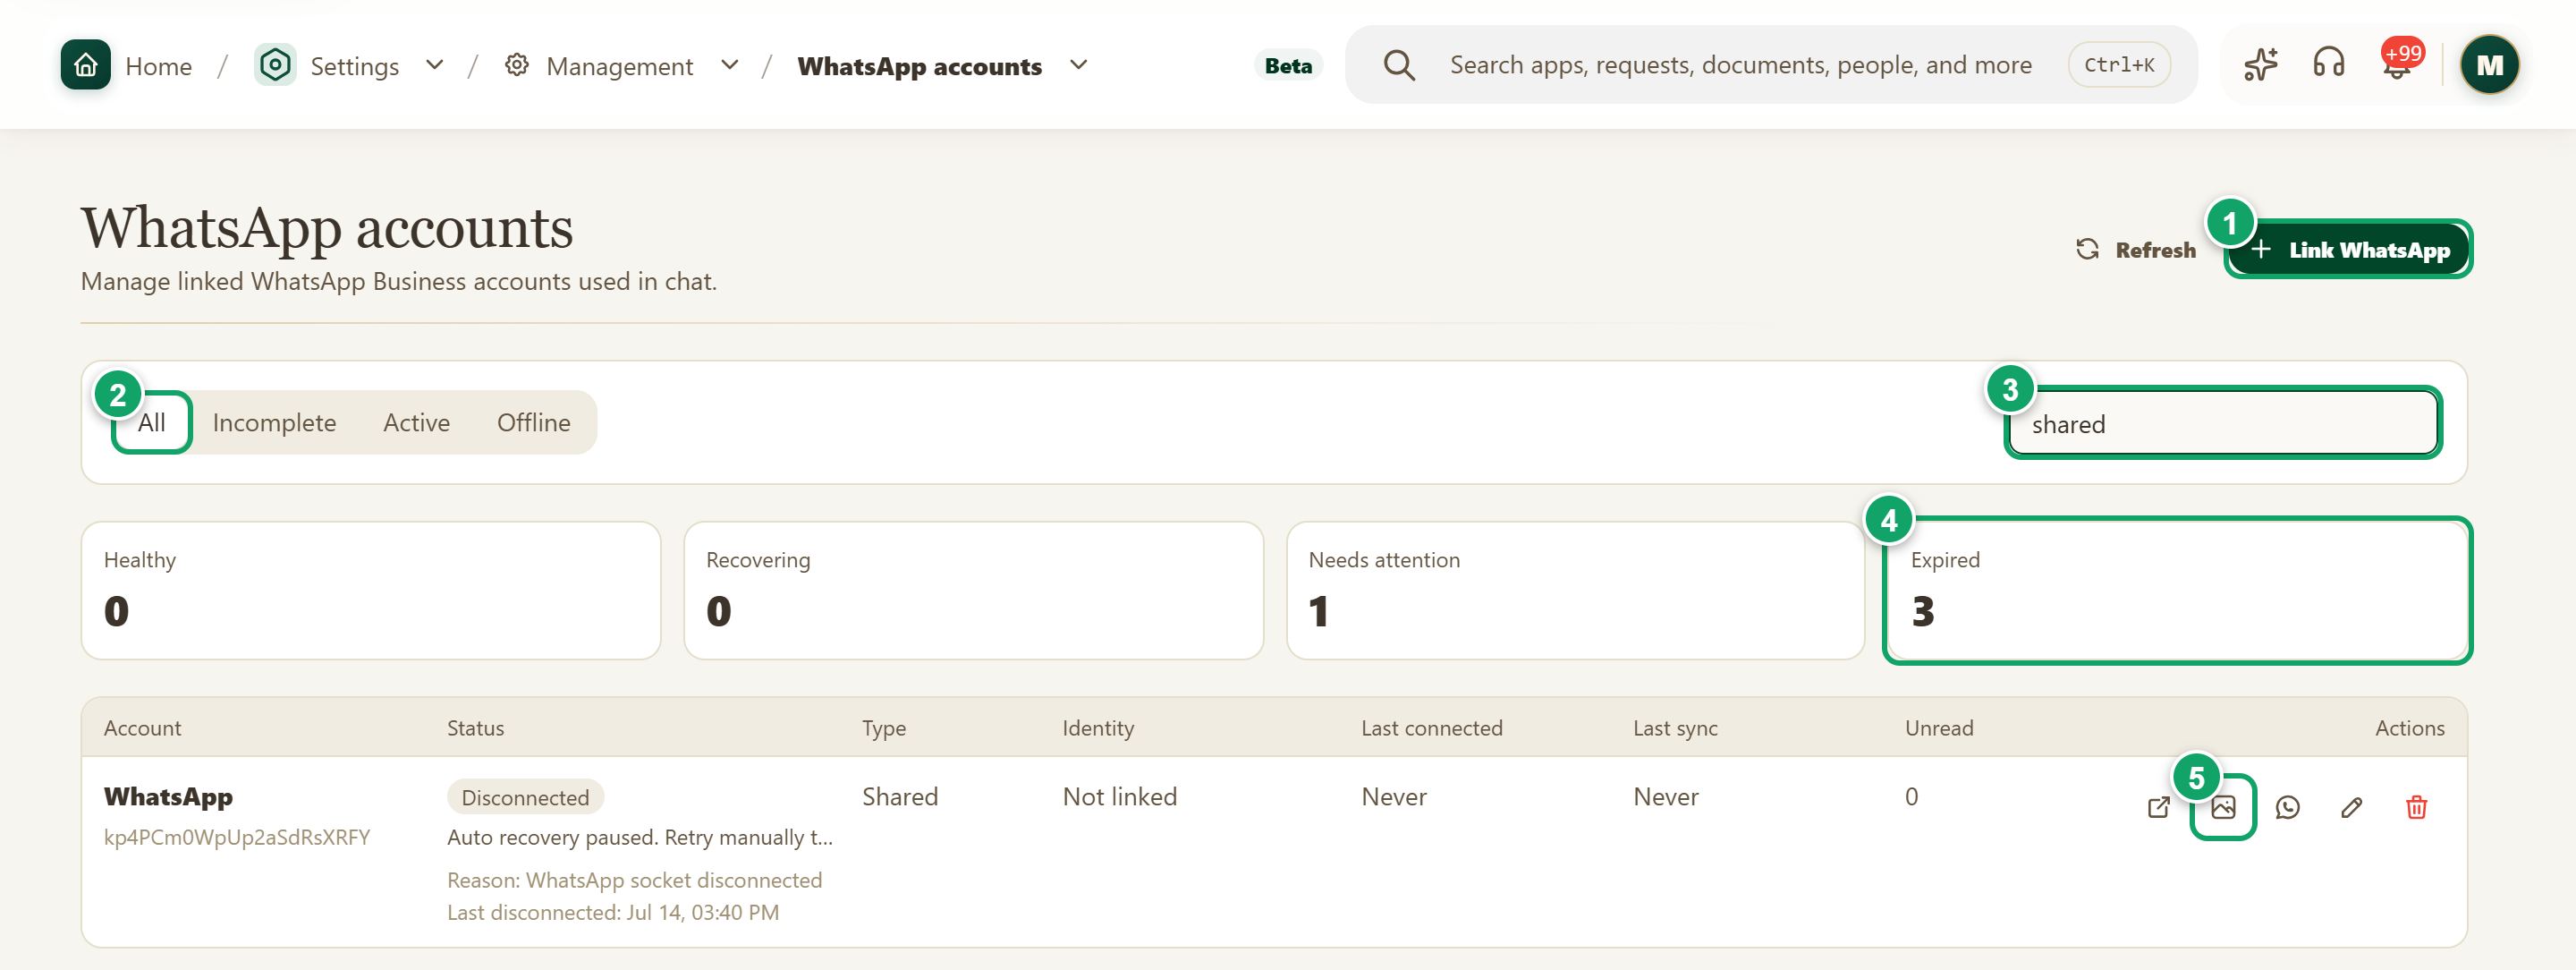
\includegraphics[width=0.95\linewidth,height=0.72\textheight,keepaspectratio]{figures/screens/ch08-whatsapp-en.png}
\caption{The WhatsApp accounts list}
\label{fig:settings-whatsapp}
\shotnote{The cards summarize the health of all accounts, while the table explains each account’s status and why it dropped. A search is applied in the image to show only the shared account, so no personal phone numbers appear; the cards still count all accounts. ① “Link WhatsApp”. ② “All”: with “Incomplete”, “Active” and “Offline”, filters the list. ③ The search field. ④ “Expired”: accounts that need relinking. ⑤ “Media status”: shows the state of images and files and what failed to download.}
\end{figure}

\begin{figure}[H]
\centering
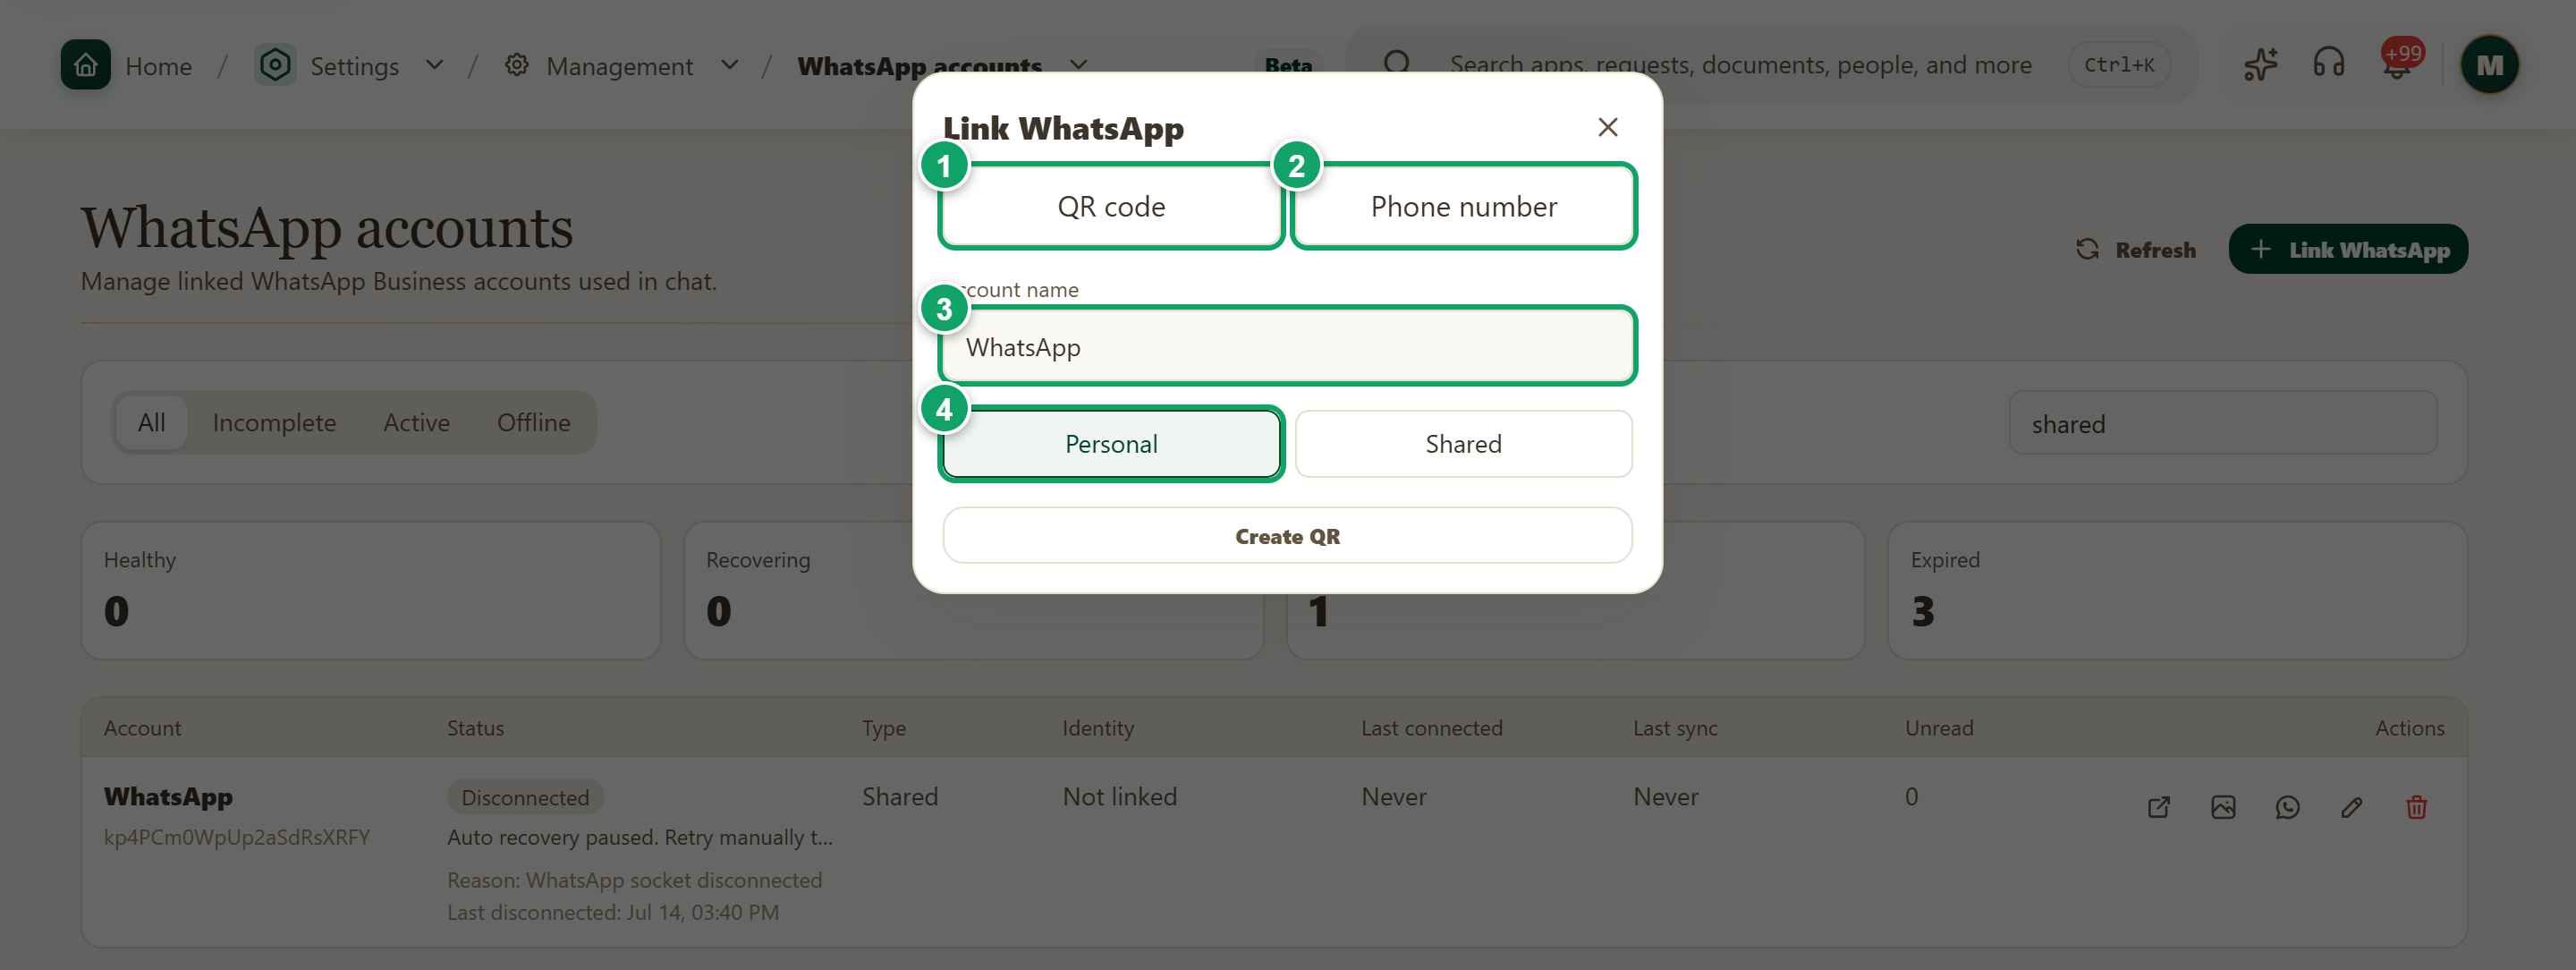
\includegraphics[width=0.95\linewidth,height=0.72\textheight,keepaspectratio]{figures/screens/ch08-whatsapp-link-en.png}
\caption{The Link WhatsApp window}
\label{fig:settings-whatsapp-link}
\shotnote{The image shows the window before linking starts, and no account was created. Linking begins only after you press the button at the bottom of the window; a code then appears that expires shortly. ① “QR code”: you scan it with the phone. ② “Phone number”: gets a pairing code you type into WhatsApp. ③ “Account name”. ④ “Personal”, with “Shared” beside it: the account type.}
\end{figure}

\begin{table}[H]
\centering
\caption{What do you record and read in WhatsApp accounts?}
\label{tab:settings-whatsapp-fields}
\begin{tabularx}{\linewidth}{R{4.2cm} Y}
\rcHeaderRow
\thh{Item} & \thh{What does it mean?}\\
When linking & The linking method, “Account name”, and the type, “Personal” or “Shared”.\\
The cards & “Healthy”, “Recovering”, “Needs attention” and “Expired”.\\
Table columns & “Account”, “Status” with the reason for dropping, “Type”, “Identity”, which is the linked number, “Last connected”, “Last sync” and “Unread”.\\
Actions & “Open in chat”, “Media status”, “Link account”, “Retry now”, “Disconnect account”, “Rename account” and “Delete account”. They appear according to the account’s state and your permission.\\
\end{tabularx}
\end{table}

\begin{enumerate}
\item Open “Settings”, then “WhatsApp accounts”, and press “Link WhatsApp”.
\item Choose “QR code” or “Phone number”.
\item Type the “Account name” and choose “Personal” or “Shared”.
\item With a code, press “Create QR”, then scan it from “Linked devices” in WhatsApp on the phone.
\item With a phone number, type it with its country code and press “Get pairing code”, then enter the code in WhatsApp. You can request one code per minute.
\end{enumerate}

\textbf{Check:} The window closes, the account appears in the table as “Active”, and “Open in chat” opens it. If “Relink required” appears, use “Link account” again. “Delete account” asks for confirmation and disconnects an active session first.
